\chapter{Arhitektura i dizajn sustava}
		
		\textbf{\textit{dio 1. revizije}}\\
		
		
		Arhitektura ovog sustava je bazirana na arhitekturi klijent-poslužitelj. Sustav se sastoji od 3 sloja: sloj korisničkog sučelja, sloj aplikacijske logike, sloj podataka.
		
		Korisnik koristi aplikaciju preko web preglednika. Web preglednik je program koji omogućuje klijentu komunikaciju s web poslužiteljem aplikacije. Preglednik nam omogućava prikaz sloja korisničkog sučelja sustava. Korisnik preko web preglednika komunicira s web poslužiteljem slanjem i primanjem HTTP zahtjeva. Primljene podatke i datoteke web preglednik zna interpretirati i prikazati korisniku tako da sama interakcija s aplikacijom bude jednostavna.
		
		Web poslužitelj je računalo na kojem se aplikacija pokreće. Na njemu se dakle nalazi sloj aplikacijske logike. Web poslužitelj aplikaciji prosljeđuje zahtjeve na obradu i njezine odgovore prosljeđuje natrag klijentima. Web aplikacija na poslužitelju obrađuje zaprimljene zahtjeve. Ako obrada zahtjeva to zahtjeva, web aplikacija dodatno komunicira sa slojem podataka.
		
		Sloj podataka je predstavljen bazom podataka. U bazi podataka se na siguran način spremaju svi podaci koje je potrebno trajno čuvati. To podrazumijeva podatke o prijavama, korisničkim računima i slično. Takvi podaci moraju ostati očuvani i ako je rad aplikacije prekinut iz bilo kojeg razloga. Baza podataka je detaljnije opisana u poglavlju  4.1.
		
		Web aplikacija je podijeljena na frontend i backend.
		
		Frontend je zapravo prezentacijski dio aplikacije. On zapravo oblikuje korisničko sučelje i samim time definira što će korisnik vidjeti na web pregledniku kada koristi aplikaciju.
		
		Backend je dio aplikacije koji obrađuje zahtjeve i kontrolira rad ostalih dijelova sustava.
		
		Arhitektura same web aplikacije je odrađena u stilu MVC arhitekture. U ovoj arhitekturi aplikacija se dijeli na 3 sloja, svaki sa svojom ulogom. Ovime se postiže podjela odgovornosti pojedinih komponenti sustava. Sama struktura aplikacije je preglednija i smislenije primjenom ove arhitekture. Također, razvoj i održavanje sustava je znatno olakšan primjenom ove arhitekture. MVC arhitektura je izuzetno popularna u razvoju web aplikacija te je stoga dobro razrađena i mnogi radni okviri podržavaju njezinu implementaciju. MVC arhitekura se sastoji od slojeva:
		\begin{packed_item}
			\item \textbf{Model} - predstavlja komponentu aplikacije koja modelira aplikacijsku logiku. Ovaj model preslikava podatke dobivene od korisnika u bazu podataka i obrnuto. Na temelju zaprimljenih podataka vrši obradu zahtjeva.
			
			\item \textbf{Pogled(View)} - predstavlja dio aplikacije zadužen az prikaz podataka korisniku. Također omogućava korisniku interakciju s aplikacijom kroz prikaz korisničkog sučelja. Usko je povezan s frontend dijelom aplikacije.
			
			\item \textbf{Upravljač(Controller)} - upravlja nadolazećim zahtjevima. Ova komponenta prosljeđuje zahtjeve modelu na obradu. Od modela zaprima odgovore koje prosljeđuje komponenti za pogled na formiranje grafičkog prikaza koje se zatim prikazuje korisniku.
		\end{packed_item}
		
		Kroz međusobnu interakciju ova 3 modela omogućuju normalno funkcioniranje aplikacije.
		
		\begin{figure}[H]
			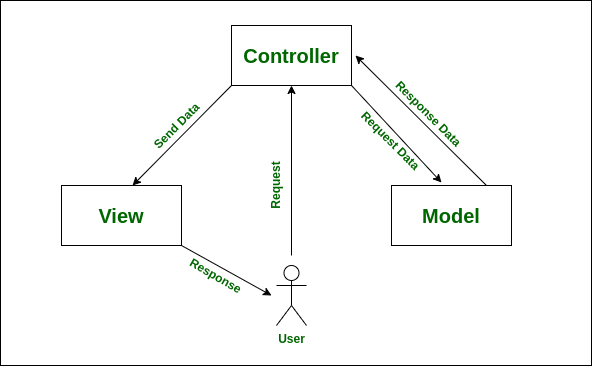
\includegraphics[width=\textwidth]{slike/mvc.png} %veličina u odnosu na širinu linije
			\caption{prikaz komponenti u MVC arhitekturi}
			\label{fig:MVC1} %label mora biti drugaciji za svaku sliku
		\end{figure}
		
		Za razvoj frontend dijela aplikacije odlučili smo koristiti programski jezik JavaScript uz radni okvir React. Backend dio aplikacije je realiziran u programskom jeziku Java uz radni okvir Spring Boot.
		

		\textit{ Potrebno je opisati stil arhitekture te identificirati: podsustave, preslikavanje na radnu platformu, spremišta podataka, mrežne protokole, globalni upravljački tok i sklopovsko-programske zahtjeve. Po točkama razraditi i popratiti odgovarajućim skicama:}
	\begin{itemize}
		\item 	\textit{izbor arhitekture temeljem principa oblikovanja pokazanih na predavanjima (objasniti zašto ste baš odabrali takvu arhitekturu)}
		\item 	\textit{organizaciju sustava s najviše razine apstrakcije (npr. klijent-poslužitelj, baza podataka, datotečni sustav, grafičko sučelje)}
		\item 	\textit{organizaciju aplikacije (npr. slojevi frontend i backend, MVC arhitektura) }		
	\end{itemize}
	\eject
	
		

		\section{Baza podataka}
			
		\textbf{\textit{dio 1. revizije}}\\
			
		Ovaj sustav će za svoje potrebe koristiti relacijsku bazu podataka implementirana u PostgreSQL-u. Ovakav tip baze podataka svojom strukturom omogućuje jednostavno modeliranje elemenata iz stvarnog svijeta i zbog toga je široko primjenjiv. Odabrali smo implementaciju u PostgreSQL-u jer smo s ovom implementacijom već dobro upoznati. Relacijske baze podataka se sastoje od relacija. Relacije su predstavljene tablicama koje su definirane svojim nazivom i skupom atributima. Bazu podataka koristimo za jednostavnu i sigurnu pohranu, izmjenu, umetanje i dohvat podataka potrebnih za rad sustava. Naša baza podataka se sastoji od sljedećih relacija, odnosno tablica:
		
		\begin{packed_item}
			\item Users
			\item Report
			\item Image
			\item Category
			\item CategoryKeywords
			\item ReportGroup 
			\item Feedback
			\item CityOffice
		\end{packed_item}
			
		\textit{Potrebno je opisati koju vrstu i implementaciju baze podataka ste odabrali, glavne komponente od kojih se sastoji i slično.}
		
			\subsection{Opis tablica}
			
			\textbf{Users} tablica čuva podatke o korisničkim računima koje korisnici izrađuju tijekom registracije. Tablica je povezana vezom \textit{One-to-Many} s tablicom \textit{Report} preko atributa \textit{userID}.
			
			\begin{longtblr}[
					label=Users,
					entry=none
				]{
					width = \textwidth,
					colspec={|X[6,l]|X[6, l]|X[20, l]|}, 
					rowhead = 1,
				} %definicija širine tablice, širine stupaca, poravnanje i broja redaka naslova tablice
				\hline \SetCell[c=3]{c}{\textbf{Users}}	 \\ \hline[3pt]
				\SetCell{LightGreen} userID & INT & jedinstveni identifikator korisnika \\ \hline
				email & VARCHAR & email adresa korisnika \\ \hline 
				firstName & VARCHAR & ime korisnika \\ \hline
				lastName & VARCHAR & prezime korisnika \\ \hline 
				password & VARCHAR & kriptirana lozinka za korisnički račun \\ \hline 
			\end{longtblr}
			
			\textbf{Report} tablica čuva podatke o pojedinim prijavama oštećenja koje korisnici podnose. Tablica je povezana vezom \textit{Many-to-One} s tablicom \textit{Users} preko atributa \textit{userID}, \textit{Many-to-One} vezom s tablicom \textit{Category} preko atributa \textit{categoryID} i \textit{Many-to-One} vezom s tablicom ReportGroup preko atributa groupID.
			
			\begin{longtblr}[
				label=Report,
				entry=none
				]{
					width = \textwidth,
					colspec={|X[8,l]|X[6, l]|X[20, l]|}, 
					rowhead = 1,
				} %definicija širine tablice, širine stupaca, poravnanje i broja redaka naslova tablice
				\hline \SetCell[c=3]{c}{\textbf{Report}}	 \\ \hline[3pt]
				\SetCell{LightGreen} reportID & INT & jedinstveni identifikator prijave \\ \hline
				location & VARCHAR & lokacija oštećenja \\ \hline
				description & VARCHAR & opis oštećenja \\ \hline 
				reportTS & TIMESTAMP & vrijeme prijave \\ \hline 
				reportHeadline & VARCHAR & naslov prijave \\ \hline 
				\SetCell{LightBlue} userID & INT & jedinstveni identifikator korisnika koji je podnio prijavu \\ \hline 
				\SetCell{LightBlue} categoryID & INT & jedinstveni identifikator kategorije oštećenja \\ \hline
				\SetCell{LightBlue} groupID & INT & jedinstveni identifikator grupe prijave \\ \hline
			\end{longtblr}
			
			\textbf{Image} tablica čuva podatke o slikama koje se prilažu u prijavama oštećenja. Tablica je povezana \textit{Many-to-One} vezom s tablicom \textit{Report} preko atributa \textit{reportID}.
			
			\begin{longtblr}[
				label=Image,
				entry=none
				]{
					width = \textwidth,
					colspec={|X[6,l]|X[6, l]|X[20, l]|}, 
					rowhead = 1,
				} %definicija širine tablice, širine stupaca, poravnanje i broja redaka naslova tablice
				\hline \SetCell[c=3]{c}{\textbf{Image}}	 \\ \hline[3pt]
				\SetCell{LightGreen} imageID & INT & jedinstveni identifikator slike \\ \hline
				\SetCell{LightBlue} reportID & INT & jedinstveni identifikator prijave kojoj slika pripada \\ \hline
				URL & VARCHAR & URL slike \\ \hline 
			\end{longtblr}
			
			\textbf{Category} tablica čuva podatke o kategorijama kojima oštećenje može pripadati. Tablica je povezana \textit{One-to-Many} vezom s tablicom \textit{Report} preko atributa \textit{categoryID}, \textit{Many-to-One} vezom s tablicom \textit{CityOffice} preko atributa \textit{cityOfficeID} i \textit{One-to-Many} vezom s tablicom \textit{CategoryKeywords} preko atributa \textit{categoryID}.
			
			\begin{longtblr}[
				label=Category,
				entry=none
				]{
					width = \textwidth,
					colspec={|X[6,l]|X[6, l]|X[20, l]|}, 
					rowhead = 1,
				} %definicija širine tablice, širine stupaca, poravnanje i broja redaka naslova tablice
				\hline \SetCell[c=3]{c}{\textbf{Category}}	 \\ \hline[3pt]
				\SetCell{LightGreen} categoryID & INT & jedinstveni identifikator kategorije \\ \hline
				categoryName & VARCHAR & naziv kategorije \\ \hline 
				\SetCell{LightBlue} cityOfficeID & INT & jedinstveni identifikator gradskog ureda koji obrađuje prijave oštećenja iz ove kategorije \\ \hline
			\end{longtblr}

			\textbf{CategoryKeywords} tablica čuva podatke o ključnim riječima po kojima se može identificirati kategorija oštećenja. Tablica je povezana \textit{Many-to-One} vezom s tablicom \textit{Category} preko atributa \textit{categoryID}.

			\begin{longtblr}[
				label=CategoryKeywords,
				entry=none
				]{
					width = \textwidth,
					colspec={|X[6,l]|X[6, l]|X[20, l]|}, 
					rowhead = 1,
				} %definicija širine tablice, širine stupaca, poravnanje i broja redaka naslova tablice
				\hline \SetCell[c=3]{c}{\textbf{CategoryKeywords}}	 \\ \hline[3pt]
				\SetCell{LightGreen} keywordID & INT & jedinstveni identifikator ključne riječi \\ \hline
				keyword & VARCHAR & ključna riječ \\ \hline 
				\SetCell{LightBlue} categoryID & INT & jedinstveni identifikator kategorije kojoj ključna riječ pripada. \\ \hline
			\end{longtblr}
			
			\textbf{ReportGroup} tablica predstavlja grupu prijava koje su objedinjene. Tablica je povezana \textit{One-to-Many} vezom s tablicom \textit{Report} preko atributa \textit{groupID} i \textit{One-to-Many} vezom s tablicom \textit{Feedback} preko atributa \textit{groupID}.
			
			\begin{longtblr}[
				label=ReportGroup,
				entry=none
				]{
					width = \textwidth,
					colspec={|X[6,l]|X[6, l]|X[20, l]|}, 
					rowhead = 1,
				} %definicija širine tablice, širine stupaca, poravnanje i broja redaka naslova tablice
				\hline \SetCell[c=3]{c}{\textbf{ReportGroup}}	 \\ \hline[3pt]
				\SetCell{LightGreen} groupID & INT & jedinstveni identifikator grupe prijava \\ \hline
			\end{longtblr}
			
			\textbf{Feedback} tablica čuva podatke o statusu pojedine grupe prijava. Također čuva podatke potrebne za slanje povratnih informacija korisnicima i računanje nekih statistika. Tablica je povezana \textit{Many-to-One} vezom s tablicom \textit{ReportGroup} preko atributa \textit{groupID} i \textit{Many-to-One} vezom s tablicom \textit{CityOffice} preko atributa \textit{cityOfficeID}.
			
			\begin{longtblr}[
				label=Feedback,
				entry=none
				]{
					width = \textwidth,
					colspec={|X[6,l]|X[6, l]|X[20, l]|}, 
					rowhead = 1,
				} %definicija širine tablice, širine stupaca, poravnanje i broja redaka naslova tablice
				\hline \SetCell[c=3]{c}{\textbf{Feedback}}	 \\ \hline[3pt]
				\SetCell{LightGreen} cityOfficeID & INT & jedinstveni identifikator gradskog ureda \\ \hline
				\SetCell{LightGreen} groupID & INT & jedinstveni identifikator grupe prijava na koju se podaci referiraju \\ \hline
				status & VARCHAR & status prijava u referiranoj grupi \\ \hline 
				changeTS & TIMESTAMP & vrijeme kada se postavio status prijava iz referirane grupe \\ \hline
			\end{longtblr}
			
			\textbf{CityOffice} tablica čuva podatke o računima gradskih ureda. Tablica je povezana \textit{One-to-Many} vezom s tablicom \textit{Feedback} preko atributa \textit{cityOfficeID} i \textit{One-to Many} vezom s tablicom \textit{Category} preko atributa \textit{cityOfficeID}.
			
			\begin{longtblr}[
				label=CityOffice,
				entry=none
				]{
					width = \textwidth,
					colspec={|X[10,l]|X[6, l]|X[20, l]|}, 
					rowhead = 1,
				} %definicija širine tablice, širine stupaca, poravnanje i broja redaka naslova tablice
				\hline \SetCell[c=3]{c}{\textbf{CityOffice}}	 \\ \hline[3pt]
				\SetCell{LightGreen} cityOfficeID & INT & jedinstveni identifikator gradskog ureda \\ \hline
				cityOfficeName & VARCHAR & naziv gradskog ureda \\ \hline
				cityOfficeEmail & VARCHAR & email adresa gradskog ureda \\ \hline 
				cityOfficePassword & VARCHAR & kriptirana lozinka za račun gradskog ureda \\ \hline
			\end{longtblr}
		
				
				
			
			\subsection{Dijagram baze podataka}
			
			\begin{figure}[H]
				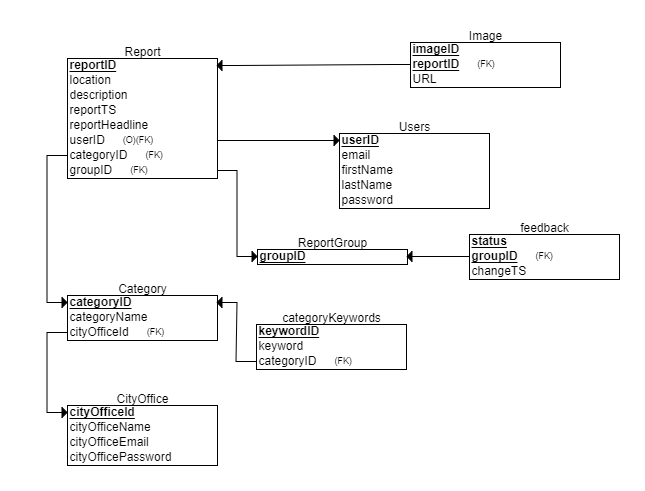
\includegraphics[width=\textwidth]{slike/relacijski.png} %veličina u odnosu na širinu linije
				\caption{relacijski dijagram baze podataka}
				\label{fig:DijagramBazePodataka} %label mora biti drugaciji za svaku sliku
			\end{figure}
			
			\eject
			
			
		\section{Dijagram razreda}
		
			\textit{Potrebno je priložiti dijagram razreda s pripadajućim opisom. Zbog preglednosti je moguće dijagram razlomiti na više njih, ali moraju biti grupirani prema sličnim razinama apstrakcije i srodnim funkcionalnostima.}\\
			
			\textbf{\textit{dio 1. revizije}}\\
			
			\textit{Prilikom prve predaje projekta, potrebno je priložiti potpuno razrađen dijagram razreda vezan uz \textbf{generičku funkcionalnost} sustava. Ostale funkcionalnosti trebaju biti idejno razrađene u dijagramu sa sljedećim komponentama: nazivi razreda, nazivi metoda i vrste pristupa metodama (npr. javni, zaštićeni), nazivi atributa razreda, veze i odnosi između razreda.}\\
			
			\textbf{\textit{dio 2. revizije}}\\			
			
			\textit{Prilikom druge predaje projekta dijagram razreda i opisi moraju odgovarati stvarnom stanju implementacije}
			
			
			
			\eject
		
		\section{Dijagram stanja}
			
			
			\textbf{\textit{dio 2. revizije}}\\
			
			\textit{Potrebno je priložiti dijagram stanja i opisati ga. Dovoljan je jedan dijagram stanja koji prikazuje \textbf{značajan dio funkcionalnosti} sustava. Na primjer, stanja korisničkog sučelja i tijek korištenja neke ključne funkcionalnosti jesu značajan dio sustava, a registracija i prijava nisu. }
			
			
			\eject 
		
		\section{Dijagram aktivnosti}
			
			\textbf{\textit{dio 2. revizije}}\\
			
			 \textit{Potrebno je priložiti dijagram aktivnosti s pripadajućim opisom. Dijagram aktivnosti treba prikazivati značajan dio sustava.}
			
			\eject
		\section{Dijagram komponenti}
		
			\textbf{\textit{dio 2. revizije}}\\
		
			 \textit{Potrebno je priložiti dijagram komponenti s pripadajućim opisom. Dijagram komponenti treba prikazivati strukturu cijele aplikacije.}